To augment the artist records, Karma first looks for R2RML mappings that describe crm:E21\_Person to discover available object and data properties to present to the user.
Karma could look in a triple store for all the properties with subjects or objects of type crm:E21\_Person or even use OWL to reason about the properties that could refer to crm:E21\_Person.
That would be exhaustive and expensive.
In the end, the user would still be overwhelmed with possibilities and have no guarantee that the properties would be meaningful.
Instead, the R2RML mappings allow Karma to identify the meaningful properties and present them to the user as illustrated in Figure~\ref{fig:search-screenshot}.
\begin{figure*}
\begin{center}
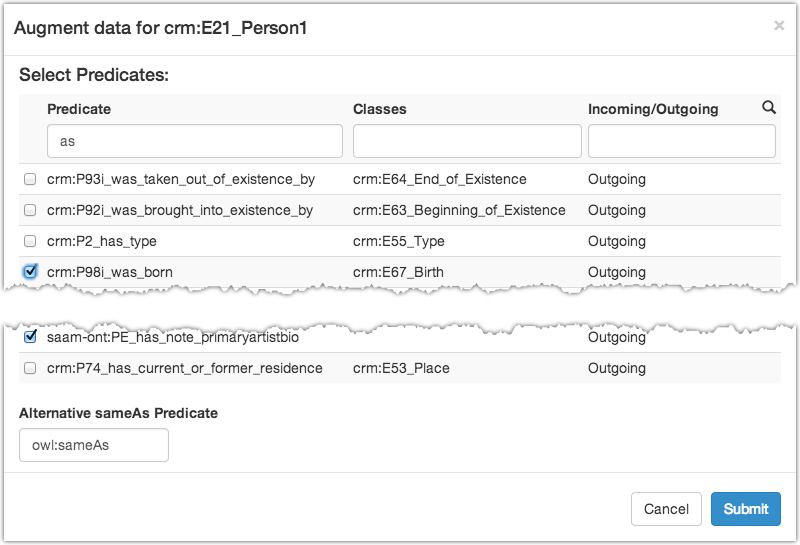
\includegraphics[width=4.9in]{images/5-search.png}
\vspace{-3mm}
\caption{A Karma user selects CIDOC CRM object and data properties discovered from other sources to augment crm:E21\_Person}
\vspace{-2mm}
\label{fig:search-screenshot}
\end{center}
\vspace{-1.5em}
\end{figure*}